\documentclass[11pt]{article}
\usepackage{ucs}
\usepackage[utf8x]{inputenc}
\usepackage{changepage}
\usepackage{graphicx}
\usepackage{amsmath}
\usepackage{gensymb}
\usepackage{amssymb}
\usepackage{enumerate}
\usepackage{tabularx}
\usepackage{lipsum}
\usepackage{amsthm}
\usepackage{thmtools}
\usepackage{float}


\usepackage{fontspec} % loaded by polyglossia, but included here for transparency 
\usepackage{polyglossia}

\usepackage{xeCJK}
\setCJKmainfont{SimSun}
%\setmainlanguage{russian} 
\setmainlanguage{latvian}
\setotherlanguage{english}

\newfontfamily\cyrillicfont[Script=Cyrillic]{Times New Roman}
\newfontfamily\cyrillicfontsf[Script=Cyrillic]{Arial}
\newfontfamily\cyrillicfonttt[Script=Cyrillic]{Courier New}

\oddsidemargin 0.0in
\evensidemargin 0.0in
\textwidth 6.27in
\headheight 1.0in
\topmargin 0.0in
\headheight 0.0in
\headsep 0.0in
%\textheight 9.69in
\textheight 9.00in
 
\setlength\parindent{0pt}

\newenvironment{myenv}{\begin{adjustwidth}{0.4in}{0.4in}}{\end{adjustwidth}}
\renewcommand{\abstractname}{Anotācija}
\renewcommand\refname{Atsauces}

%\newenvironment{uzdevums}[1][\unskip]{%
%\vspace{3mm}
%\noindent
%\textbf{#1:}
%\noindent}
%{}


% http://tex.stackexchange.com/questions/196961/thmtools-declaration-for-theorem-and-proof
\declaretheoremstyle[headfont=\normalfont\bfseries,notefont=\mdseries\bfseries,bodyfont = \normalfont,headpunct={:}]{normalhead}
\declaretheorem[name={Uzdevums}, style=normalhead,numberwithin=section]{problem}

\def\changemargin#1#2{\list{}{\rightmargin#2\leftmargin#1}\item[]}
\let\endchangemargin=\endlist 


\newcommand{\subf}[2]{%
  {\small\begin{tabular}[t]{@{}c@{}}
  #1\\#2
  \end{tabular}}%
}



\newcounter{alphnum}
\newenvironment{alphlist}{\begin{list}{(\Alph{alphnum})}{\usecounter{alphnum}\setlength{\leftmargin}{2.5em}} \rm}{\end{list}}

\newenvironment{zhtext}{\fontfamily{MS PGothic}\selectfont}{\par}


\makeatletter
\let\saved@bibitem\@bibitem
\makeatother

\usepackage{bibentry}
%\usepackage{hyperref}

\newenvironment{tulkojums}[1][\unskip]{%
\begin{changemargin}{8mm}{8mm}
\fontsize{9}{11}
\selectfont
\textbf{#1:}
}
{ 
\fontsize{12}{14}
\selectfont
\end{changemargin}
}

\setcounter{section}{0}


\begin{document}

\begin{center}
{\Large \bf Atlases sacensības komandu olimpiādei ``Baltijas ceļš''}\\
{\bf 2019.\ gada 21.\ septembris, Rīga (1.\ diena)}
\end{center}

{\footnotesize \em 
Risināšanas laiks: 4 stundas un 30 minūtes.\\
Jautājumus drīkst uzdot pirmo 60 minūšu laikā.\\ 
Atļauts izmantot tikai rakstāmpiederumus, lineālu un cirkuli.
}

\begin{problem}[BW.TST.2019.1]
Reāliem pozitīviem skaitļiem $a$, $b$ un $c$ ir spēkā sakarība 
$\frac{1}{a} + \frac{1}{b} + \frac{1}{c} = 1$. Pierādiet, ka 
\[ 3(ab + bc + ca) + \frac{9}{a+b+c} \leq \frac{9abc}{a+b+c} + 2\left( a^2 + b^2 + c^2 \right) + 1, \]
un noskaidrojiet, kādiem $a,b,c$ izpildās vienādība.
\end{problem}


\begin{problem}[BW.TST.2019.2]
Atrast visas funkcijas $f\,:\,\mathbb{R}\,\rightarrow\,\mathbb{R}$, kas definētas reāliem skaitļiem, 
pieņem reālas vērtības un kurām visiem reāliem $x$ un $y$ ir spēkā vienādība
\[ f\left( y^2 - f(x) \right) = yf(x)^2 + f(x^2y + y). \]
\end{problem}

\begin{problem}[BW.TST.2019.3]
Sienāzis lēkā pa veselo skaitļu asi. Tas sāk savu ceļu tās sākumpunktā ($x = 0$) 
un katrā lēcienā var lēkt vai nu pa labi, vai pa kreisi, pie tam sienāža $n$-tā 
lēciena garums ir tieši $n^2$.\\
Pierādiet, ka sienāzis var nokļūt jebkurā (veselā) skaitļu ass punktā. 
\end{problem}

\begin{problem}[BW.TST.2019.4]
Dots $n$-tās pakāpes polinoms $P(x)$ ar reāliem koeficientiem, kuram visiem 
$0 \leq y \leq 1$ izpildās $|p(y)| \leq 1$. 
Pierādīt, ka $p\left( \frac{1}{n} \right) \leq 2^{n+1} - 1$.
\end{problem}


\begin{problem}[BW.TST.2019.5]
Aplī nostājušies $2019$ pirmklasnieki, sākumā katram rokās ir tieši viena gladiola. 
Katrā gājienā skolotāja izvēlas vienu pirmklasnieku, kuram rokās ir vismaz viena gladiola, 
un tas vienu savu gladiolu atdod savam kaimiņam vai nu pa labi, vai pa kreisi. 
Pierādīt, ka neatkarīgi no skolotājas darbībām pirmklasnieki var (saskaņoti) rīkoties 
tā, lai nevienā brīdī nevienam pirmklasniekam rokās nebūtu vairāk kā divas gladiolas.
\end{problem}

\begin{problem}[BW.TST.2019.6]
Vectēvam bēniņos ir galīgs skaits tukšu kartona kastu, katra kaste ir taisnstūra
paralēlskaldnis, kura malu garumi ir naturāli skaitļi. 
Katrai kastei platums nav lielāks kā garums un augstums nav lielāks kā platums. 
Vienu kartona kasti var ievietot otrā kastē, ja pirmās kastes  garums, platums un augstums 
ir attiecīgi mazāki nekā otrās kastes garums, platums un augstums. Vienā kastē var ielikt divas vai 
vairāk akstes tikai tad, ja tās ir ieliktas viena otrā. 

Vectēvs nolēma savas kastes salikt vienu otrā tā, lai viņam bēniņos paliktu pēc iespējas 
mazāks skaits kastu (kas nav ieliktas kādā citā kastē). Viņš rīkojās pēc šāda algoritma: 
katrā solī viņš atrada tādu garāko kastu virkni, ka tās var
ielikt pirmo otrajā, otro trešajā, utt. un salika tās vienu otrā, tad šo procesu 
atkārtoja līdz brīdim, kad nevienu kasti vairs nevarēja ielikt nevienā citā. 
Katrā solī vectēvam šī garākā kastu virkne, ko viņš salika vienu otrā, bija 
unikāla, t.i. nevienā solī nebija vairāku virkņu ar vienādiem garumiem. 
Vai var droši apgalvot, ka tagad vectēvam bēniņos ir mazākais iespējamais skaits kastu
(kas nav ieliktas nevienā citā kastē)?
\end{problem}

\begin{problem}[BW.TST.2019.7]
Dotas divas virknes $b_i, c_i$, $0 \leq i \leq 100$, kuru locekļi ir naturāli 
skaitļi, izņemot $c_0 = 0, b_{100} = 0$. 

Daži ciemati Graflandē ir savienoti ar ceļiem, pie kam katrs ceļš savieno 
tieši divus ciematus, ceļi ārpus ciematiem nekrustojas (bet, iespējams, 
šķērso viens otru ar viaduktu), un katrs ceļš ir 
tieši 1 km garš. Ciematus, kas ir savienoti ar ceļu, sauksim par 
{\em kaimiņiem}. Par {\em attālumu} starp ciematiem $X$ un $Y$ sauksim 
īsākā ceļa garumu, pa kuru var nonākt no $X$ uz $Y$. 

Graflandē lielākais attālums starp ciematiem ir 100 km. Tāpat ir zināma 
sekojoša īpašība: katram ciematu pārim $(X,Y)$ (iespējams, ka $X = Y$), 
ja attālums starp $X$ un $Y$ ir $k$ km, tad $Y$ ir tieši $b_k$ kaimiņi, 
kas atrodas attālumā $k+1$ no $X$, un tieši $c_k$ kaimiņi, kas 
atrodas attālumā $k-1$ no $X$. 

Pierādiet, ka 
\[ \frac{b_0b_1 \cdots b_{99}}{b_1b_2 \cdots b_{100}} \]
ir naturāls skaitlis!
\end{problem}

\begin{problem}[BW.TST.2019.8]
Vienā no $20 \times 20$ rūtiņu lapas rūtiņām ir apslēpti dārgumi. 
Lai atrastu šos dārgumus, mēs šobrīd varam pasūtīt vairākus ģeoloģiskus
pētījumus, kuru rezultāti tiks saņemti visi vienlaicīgi pēc mēneša. 
Katram pētījumam nepieciešams norādīt vienu $1 \times 4$ rūtiņu laukumu un 
pētījuma rezultātā mēs uzzināsim, vai šajā laukumā ir dārgumi, vai nav. 
Šis $1 \times 4$ rūtiņu laukums var būt novietots gan horizontāli, 
gan vertikāli un tas var arī iet pāri laukuma malai, tādā gadījumā tas
``cikliski''turpinās pretējā pusē (Att.\ 1). 

Kāds ir mazākais pētījumu skaits, kas jāpasūta, lai droši varētu noskaidrot, 
kur atrodas dārgumi?

\begin{figure}[H]
\centerline{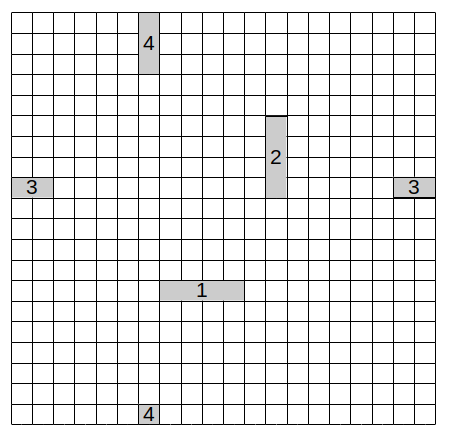
\includegraphics[width=2.5in]{Pictures/bw-tst-2019-8.png}}
\caption{Četri piemēri, kā var būt novietots $1 \times 4$ rūtiņu laukums, kurā 
tiek veikts pētījums}
\label{fig:01}
\end{figure}
\end{problem}




\begin{center}
{\bf 2019.\ gada 22.\ septembris, Rīga (2.\ diena)}
\end{center}

\begin{problem}[BW.TST.2019.9]
Dots rombs $ABCD$, zināms, ka $\sphericalangle ABC > 90^{\circ}$. 
Riņķa līnijas $\Gamma_{B}$ centrs ir punkts $B$ un tā iet caur
punktu $C$, bet riņķa līnijas $\Gamma_C$ centrs ir punkts $C$ un tā
iet aur punktu $B$. Vienu no riņķa līniju 
$\Gamma_B$ un $\Gamma_C$ krustpunktiem apzīmēsim ar $E$, 
taisne $ED$ vēlreiz krusto riņķa līniju $\Gamma_B$ punktā $F$. 
Atrodiet leņķa $\sphericalangle AFB$ vērtību. 
\end{problem}

\begin{problem}[BW.TST.2019.10]
Šaurleņķa trijstūra $ABC$ augstumi krustojas punktā $H$, malas $BC$ viduspunkts ir $M$. 
Riņķa līnijas $\omega_1$ diametrs ir $AH$, riņķa līnijas $\omega_2$ centrs ir $M$ un tā 
iekšēji pieskaras trijstūra $ABC$ apvilktajai riņķa līnijai. Pierādīt, ka 
riņķa līnijas $\omega_1$ un $\omega_2$ pieskaras viena otrai.
\end{problem}

\begin{problem}[BW.TST.2019.11]
Regulāram $2018$-stūrim $A_1A_2\ldots{}A_{2018}$ apvilktās riņķa līnijas rādiuss ir $R$. 
Pierādīt, ka 
\[ A_1A_{1008} - A_1A_{1006} + A_1A_{1004} - A_1A_{1002} + \ldots A_1A_4 - A_1A_2 = R. \]
\end{problem}

\begin{problem}[BW.TST.2019.12]
No punkta $A$ Pret riņķa līniju $\omega$ novilktas pieskares $AX$ un $AY$
($X$ un $Y$ ir pieskaršanās punkti). 
Uz nogriežņiem $AX$ un $AY$ izvēlēti attiecīgi punkti $B$ un $C$ tā, ka 
trijstūra $ABC$ perimetrs ir vienāds ar nogriežņa $AX$ garumu. Punktam $A$ simetriskais
punkts attiecībā pret taisni $BC$ ir $D$. Pierādīt, ka trijstūrim $BDC$ apvilktā riņķa
līnija pieskaras riņķa līnijai $\omega$. 
\end{problem}

\begin{problem}[BW.TST.2019.13]
Ar $s(k)$ apzīmēsim naturāla skaitļa $k$ ciparu summu. Pierādīt, ka ir bezgalīgi daudz 
tādu naturālu skaitļu $n$, kas nedalās ar $10$ un kuriem $s\left( n^2 \right) < s(n) - 5$. 
\end{problem}

\begin{problem}[BW.TST.2019.14]
Dots naturāls skaitlis $m$ un pirmskaitlis $p$, kas ir skaitļa $m^2 - 2$ dalītājs. 
Zināms, ka eksistē tāds naturāls skaitlis $a$, ka $a^2 + m -2$ dalās ar $p$. 
Pierādīt, ka eksistē tāds naturāls skaitlis $b$, ka $b^2 - m - 2$ dalās ar $p$.
\end{problem}

\begin{problem}[BW.TST.2019.15]
Atrodiet visus veselu skaitļu trijniekus $(a,b,c)$, kuriem 
\[ (a-b)^3(a+b)^2 = c^2 + 2(a-b) + 1. \]
\end{problem}

\begin{problem}[BW.TST.2019.16]
Atrodiet visus naturālu skaitļu četriniekus $(x,y,z,t)$, kuri apmierina 
sekojošu vienādojumu sistēmu
\[ \left\{
\begin{array}{l}
xyz = t!\\
(x+1)(y+1)(z+1) = (t+1)!
\end{array} \right. \]
\end{problem}


\end{document}


